 \documentclass{beamer}
\usetheme{Berlin}
\usecolortheme{beaver}
\usepackage[ngerman]{babel}
\usepackage{graphicx}
\usepackage[utf8]{inputenc}
\usepackage{times}
\usepackage[T1]{fontenc}
\usepackage{subfigure}
\usepackage{moreverb}

\title{Project R5: Eclipse view for task executions}
\author[]{Samy Dafir\\Dominik Baumgartner\\ Sophie Reischl }
\date{\today}
\begin{document}
\frame{\titlepage}

\begin{frame}
    \frametitle{Content} 
    \tableofcontents 
\end{frame}

\section{Aufgabenstellung}
\begin{frame}
	\frametitle{Aufgabenstellung}
    \begin{block}{Aufgabe:}
	    \begin{itemize}
		    \item Eclipse Plugin
		    \item Daten aus Files einlesen, diese dann grafisch darstellen 
            \item Mittels Nebula XY Graph            
	    \end{itemize}
    \end{block}
\end{frame}
\begin{frame}
	\frametitle{Data Files}
    \begin{block}{Binary File:}
	    \begin{itemize}
		    \item Data von Typ:\\
			\text{typedef struct monRec \{ }\\
			\text{\qquad double timeStamp;}\\
			\text{\qquad double value;}\\
			\text{\qquad double ID;}\\
			\text{\} MON\_RECORD;}\\
		    \item Jedes file: $Tasks\_<name\_of\_core>.vdt$
	    \end{itemize}
    \end{block}
\end{frame}

\begin{frame}
	\frametitle{Data Files}
	\begin{block}{XML File:}
			\text{<actor name="'Core\_A1"'  type="'CPUSCHEDULER"'' ID="'2"'>}\\
			\text{\quad <itemlist type="'Task"' nrOfItems=“2"'>}\\
			\text{\quad\quad <item name="'Task\_LET\_DRV\_TASK\_A1"'>}\\
			\text{\quad\quad\quad <itemAttribute name="'ID"' value="'1"' />}\\
			\text{\quad\quad\quad <property name="'Priority"' value="'10"' />}\\
			\text{\quad\quad </item>}\\
			\text{\quad\quad <item name="'Task\_A1\_10msT1\_LET01"'>}\\
			\text{\quad\quad\quad <itemAttribute name="'ID"' value="'2"' />}\\
			\text{\quad\quad\quad <property name="'Priority"' value="'5"' />}\\
			\text{\quad\quad </item>}\\
			\text{\quad </itemlist>}\\	
			\text{</actor>}\\			
	\end{block}
\end{frame}

\begin{frame}
	\frametitle{User Eingaben:}
	\begin{block}{XML File:}
		\begin{itemize}
			\item Benutzer wählt binary files und xml files
			\item Danach werden die gewünschten Tasks ausgewählt
			\item Graph mit gewählten Tasks wird erstellt
		\end{itemize}	
	\end{block}
\end{frame}

\begin{frame}
	\frametitle{Display Output:}
	\begin{block}{Graph:}
		\begin{itemize}
			\item Graph in Cores eingeteilt
			\item Jeder Task nach Priorität in Cores eingeteilt
			\item Benutzer kann zoomen auf der Zeitachse
		\end{itemize}	
	\end{block}
\end{frame}

\section{Implementation}
\begin{frame}
	\frametitle{Implementation}
	\begin{block}{What do we start with?}
		xml file: task name, id, priority
		binary files: id, states, tiestamps
	\end{block}
\end{frame}

\begin{frame}
	\begin{block}{What is there to do?}
		\begin{enumerate}
			\item Parse xml file
			\item Select processes from list
			\item Parse binary files $\rightarrow$ extract state info
			\item Map process to all its states
			\item Insert all processes into xy Graph
		\end{enumerate} 
	\end{block}
\end{frame}

\begin{frame}
	\frametitle{Parse XML}
	\begin{itemize}
		\item Parse xml with simple DOM parser.\\
		\item Create HashMap of all processes.\\ 
	\end{itemize}
	
	\begin{tabular}{|c|c|}
		\hline 
		\textbf{Taskname} & \textbf{TaskInfo} \\ 
		\hline 
		Taskname 1 & id = 4, priority = 8 \\ 
		\hline 
		Taskname 2 & id = 2, priority = 4 \\ 
		\hline 
		Taskname 3 & id = 3, priority = 9  \\ 
		\hline 
		...    & ...  \\ 
		\hline 
	\end{tabular} 
\end{frame}

\begin{frame}
	\frametitle{Parse binary files}
	Only get relevant info: Processes the user selected
	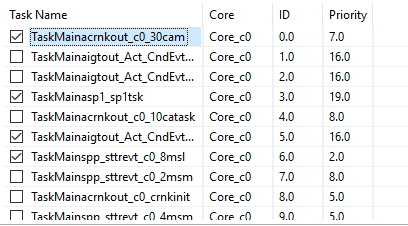
\includegraphics[width = 7cm]{table.png}
\end{frame}

\begin{frame}
	\frametitle{Parse binary files}
	\begin{block}{}
		\begin{itemize}
			\item Get selected ids from HashMap 
			\item Go through complete binary file
			\item Read state and timestamp info
			\item Only record states if ID selected
			\item All states for ID collected in HashMap
		\end{itemize}
	\end{block}
\end{frame}

\begin{frame}
	\frametitle{Parse binary files}
	\textbf{Resulting HashMap:}\\
	\vspace{1cm}
\begin{tabular}{|c|c|}
		\hline 
		\textbf{ID} & \textbf{StateInfo}  \\
		\hline 
		1 & List(states, timestamps) \\
		\hline 
		2 & List(states, timestamps)  \\ 
		\hline 
		... & ...  \\ 
		\hline 
	\end{tabular}
\end{frame}

\begin{frame}
	\frametitle{Combine process and state info}
	\begin{block}{Combine State and TaskInfo}
		\begin{itemize}
			\item contains all relevant info
			\item TreeMap provides instrinsic sorting
			\item Prefill set with TaskInfo
			\item For each entry: get States from HashMap
		\end{itemize}
	\end{block}
	\vspace{2mm}
	\begin{tabular}{|c|c|}
		\hline 
		\textbf{TraceInfo}  \\
		\hline 
		name1, core1, priority1, stateList1 \\
		\hline 
		name2, core2, priority2, stateList2  \\ 
		\hline 
		...  \\ 
		\hline 
	\end{tabular}
\end{frame}

\begin{frame}
	\frametitle{Build graph}
	\begin{block}{}
		\begin{itemize}
			\item Traces sorted by core and priority
			\item Traces contain states (1-4)
			\item Iterate over tree
			\item Calculate offset for each task
			\item Add to graph
		\end{itemize}
	\end{block}
\end{frame}




\begin{frame}
\section{Beispiel}
	\frametitle{Beispiel:}
\begin{block}{}
\end{block}
\end{frame}
\end{document}
